\documentclass[dvips,a4paper,12pt]{article}
    % \renewcommand\bibname{References} % report: Reference new page
    \renewcommand\refname{Reference} % article: Reference same page
\usepackage{xcolor}
\usepackage{float}
\usepackage{graphicx}
    \graphicspath{ {./img/} }
\usepackage[
    top=0.6in,
    bottom=0.6in,
    right=0.6in,
    left=0.6in]{geometry}

\begin{document}
\pagenumbering{arabic}


% ----------------------------------------- Begin content --------------------------------------------- %
%%% letter
\noindent Respected Examiner,

\noindent Thank you for reviewing my thesis.

\begin{center}
    \textbf{Thesis Title: Implementation of an Autonomous Star Recognition Algorithm using Hardware-Software Co-processing Approach} 
\end{center}

\noindent Firstly, I would like to thank you for your insightful comments. These excellent comments have helped significantly improve my thesis. This letter addresses each of the raised points and notes precisely how I have responded and included the comments into my revised thesis. \\

\vspace{0.5in}

\noindent Sincerely yours,

\noindent Dang Le Dang Khoa

%%% Q&A
\newpage

\color{blue}
\noindent \large{\textbf{Examiner: 1}}

\begin{enumerate}
    \color{blue}
    \item There are some obvious typos and format problems in the thesis. For example, in Page 7, the caption ‘table 2.1’ is written, but the whole table is given in Page 8. Please check and correct them.

    \color{black}
    Thanks for pointing these out. In my previous submission, while fixing some typos, I forgot to check the configuration of the LaTeX compiler leads to missing table captions.

    I have checked and fixed them all. \\

    \begin{figure}[H]
        \centering
        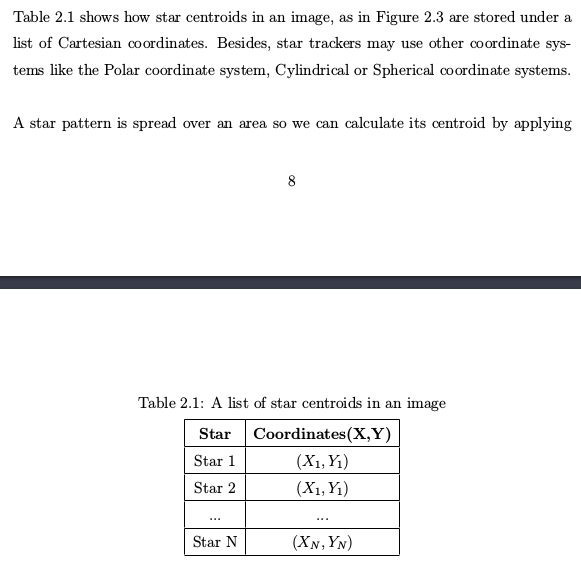
\includegraphics[width=0.6\textwidth]{1}
    \end{figure}

    \color{blue}
    \item In this thesis, the author shows some figures such as Fig. 2.2, 2.3 without any explanation. Please add some explanation to these figures in the thesis content.

    \color{black}
    Thanks for pointing out again. I have added explanations of those figures in pages 7 and 8
    
    \begin{figure}[H]
        \centering
        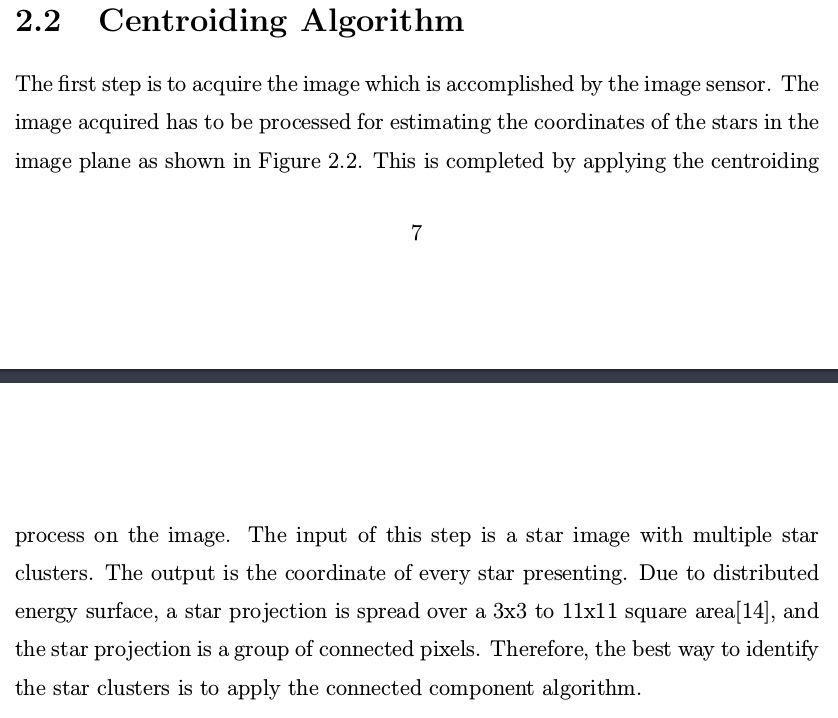
\includegraphics[width=0.6\textwidth]{2}
    \end{figure}

    \begin{figure}[H]
        \centering
        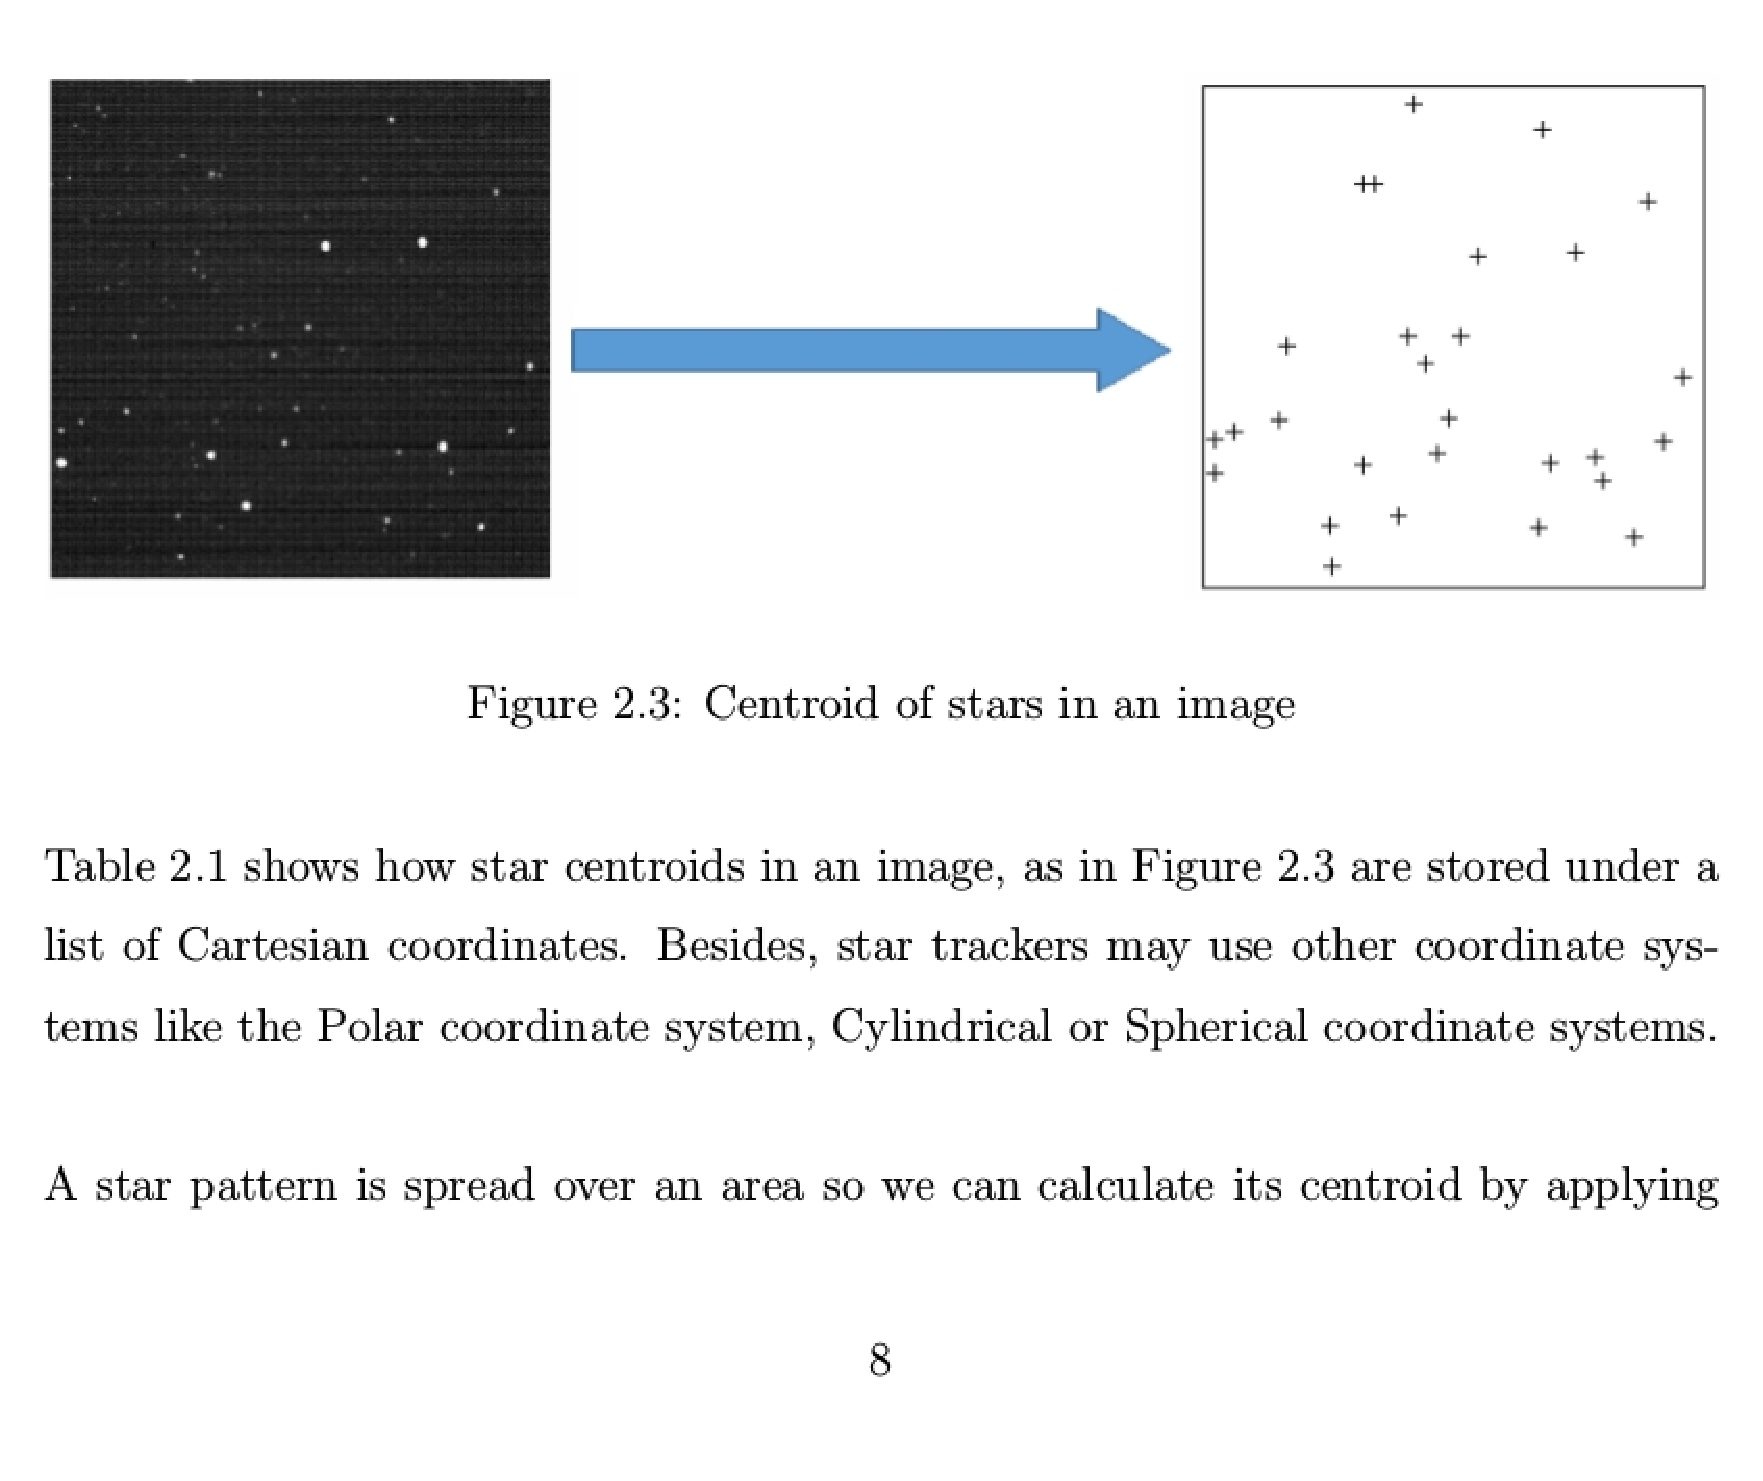
\includegraphics[width=0.6\textwidth]{3}
    \end{figure}

    \color{blue}
    \item In Chapter 3.3.1, the author applied thresholding technique in order to eliminate the noise and separate star clusters from the background. But the author did not explain how to choose the threshold.

    \color{black}
    I have amended a precise explanation to chapter 3.3.1 Centroiding (pages: 28,29,30). To summarize how to choose the threshold value:

    \begin{itemize}
        \item Firstly, I perform an analysis by averaging and counting the occurences of all pixel values in the star image dataset. 
        \item The result of the analysis would form a pattern which is shown like the below image. It includes 2 significant clusters: the first cluster is the background pixel values which formed near 0 Intensity value and the second cluster is the star pixel value which formed near the 255 Intensity value and scattered data points in between(which represent the noise)
        \item Based on the analysis, We know the range of threshold value is in between the noise values and the star pixel cluster.
        \item Finally, while carrying out experiments on the test dataset, we fine-tune and optimize the threshold value to produce the highest possible accuracy.
    \end{itemize}


    \begin{figure}[H]
        \centering
        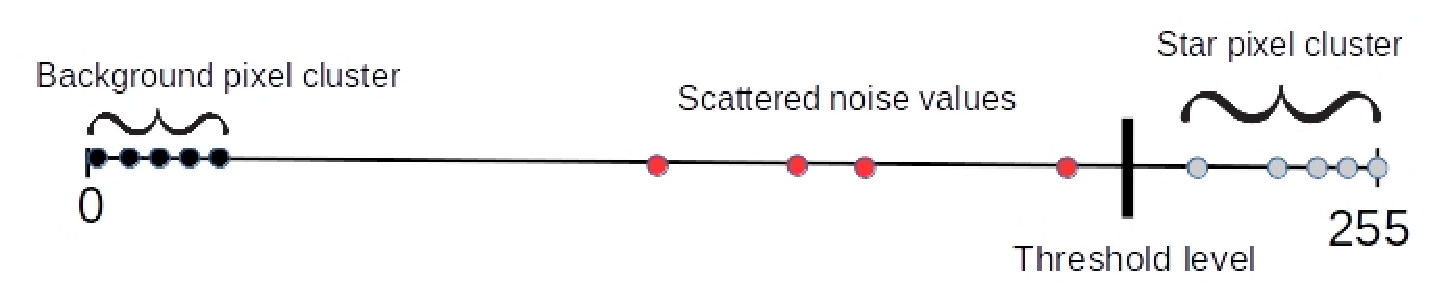
\includegraphics[width=1.0\textwidth]{4}
    \end{figure}

    \color{blue}
    \item The author claimed that the proposed prebuilt tree structured star pattern database (SPD) was able to reduce space complexity while maintaining high accuracy and robustness, so this optimized algorithm could be used for nanosatellites which have limited memory. However, there is no comparison between the SPD algorithm and traditional algorithm on accuracy, storage consumption, and robustness in this thesis.

    \color{black}
    The advantages of the proposed prebuilt tree structured star pattern database (SPD) over traditional algorithms in terms of space complexity, accuracy and robustness have been studied and proved by the previous research ``An Autonomous Star Recognition Algorithm with Optimized Star Catalogue for Fast Search Performance''\cite{MDP}.

    \color{blue}
    \item In Chapter 4.2, the author compares runtime spent by traditional methods and the proposed method in this thesis. He lists specific software runtime and hardware – software co-processing runtime when the same image dataset is used. Details of images used in experiments are also provided. However, the author only lists tables and figures to show image specifications and runtime. He does not give even one word to explain or conclude his experiment results.

    \color{black}
    I have amended detailed explanations to Chapter ``Runtime experiments'' (restructured to Chapter 4.3) from page 49 to page 56.

    \newpage
    \color{blue}
    \item In Chapter 4.1, the author gives experiment results showing hardware consumption and power consumption when the proposed method is applied. But he does not give comparison on consumption between traditional methods and his own method, therefore, readers do not know how to evaluate his experiment results. If he could add experiment results about power and hardware consumption when traditional methods are used (under the same experimental conditions), and then give a comparison between traditional methods and his method, the advantages of his proposed method would be clearer.

    \color{black}
    In Chapter Hardware design(restructured to Chapter 4.2 from page 45 to page 48), I have performed a Power Analysis of the design and proved that the Processing System (the ARM A9 processor) consumes 77\% of the power supplied while the Programmable Logic consumes 23\% of the total power. To clarify, the power consumption is measured indirectly through the number of hardware components (Logic gates, Lookup Tables, BRAM, etc.) used for the implementation and the specification of the processor (ARM A9), not directly through experiments. Therefore, I can only compare the power consumption between running an algorithm on hardware and running an algorithm on software. Based on the Power Analysis of the design, we can imply the hardware-software co-processing approach is advantageous than the software-only approach in term of power consumption. \\
    In my thesis, the parts I implemented on hardware are the DMA Data Streaming and the Centroiding modules which are the common tasks for all star tracking algorithms. Therefore, A comparison in term of power consumption between the traditional methods and the proposed method is redundant.

\end{enumerate}

%%% References
\color{black}
\bibliography{bib_reference}
\bibliographystyle{plain}

% ----------------------------------------- End content --------------------------------------------- %
\end{document}
